% ****** Start of file apssamp.tex ******
%
%   This file is part of the APS files in the REVTeX 4.1 distribution.
%   Version 4.1r of REVTeX, August 2010
%
%   Copyright (c) 2009, 2010 The American Physical Society.
%
%   See the REVTeX 4 README file for restrictions and more information.
%
% TeX'ing this file requires that you have AMS-LaTeX 2.0 installed
% as well as the rest of the prerequisites for REVTeX 4.1
%
% See the REVTeX 4 README file
% It also requires running BibTeX. The commands are as follows:
%
%  1)  latex apssamp.tex
%  2)  bibtex apssamp
%  3)  latex apssamp.tex
%  4)  latex apssamp.tex
%
\documentclass[%
 reprint,
%superscriptaddress,
%groupedaddress,
%unsortedaddress,
%runinaddress,
%frontmatterverbose, 
%preprint,
%showpacs,preprintnumbers,
%nofootinbib,
%nobibnotes,
%bibnotes,
 amsmath,amssymb,
 aps,
%pra,
%prb,
%rmp,
%prstab,
%prstper,
%floatfix,
10.5pt,
]{revtex4-1}

\usepackage{graphicx}% Include figure files
\usepackage{subfigure}
\usepackage{multirow}
\usepackage{array}
\usepackage{dcolumn}% Align table columns on decimal point
\usepackage{bm}% bold math
%\usepackage{hyperref}% add hypertext capabilities
%\usepackage[mathlines]{lineno}% Enable numbering of text and display math
%\linenumbers\relax % Commence numbering lines

%\usepackage[showframe,%Uncomment any one of the following lines to test 
%%scale=0.7, marginratio={1:1, 2:3}, ignoreall,% default settings
%%text={7in,10in},centering,
%%margin=1.5in,
%%total={6.5in,8.75in}, top=1.2in, left=0.9in, includefoot,
%%height=10in,a5paper,hmargin={3cm,0.8in},
%]{geometry}

\usepackage{xeCJK}
%\setCJKmainfont[ItalicFont={KaiTi}, BoldFont={KaiTi}]{KaiTi}
\usepackage{textcomp}
\usepackage{chemfig}
\usepackage[version=4]{mhchem}
\usepackage{fontspec}
\usepackage{listings}
\usepackage{xcolor}
\usepackage{xcolor} % 定制颜色
\definecolor{mygreen}{rgb}{0,0.6,0}
\definecolor{mygray}{rgb}{0.5,0.5,0.5}
\definecolor{mymauve}{rgb}{0.58,0,0.82}
\lstset{
backgroundcolor=\color{white},      % choose the background color
basicstyle=\footnotesize\ttfamily,  % size of fonts used for the code
columns=fullflexible,
tabsize=4,
breaklines=true,               % automatic line breaking only at whitespace
captionpos=b,                  % sets the caption-position to bottom
commentstyle=\color{mygreen},  % comment style
escapeinside={\%*}{*)},        % if you want to add LaTeX within your code
keywordstyle=\color{blue},     % keyword style
stringstyle=\color{mymauve}\ttfamily,  % string literal style
frame=single,
rulesepcolor=\color{red!20!green!20!blue!20},
% identifierstyle=\color{red},
language=Mathematica,
}

\usepackage[normalem]{ulem}

\newcommand{\chuhao}{\fontsize{42pt}{44.9pt}\selectfont}    % 初号, 1.5倍行距
\newcommand{\xiaochu}{\fontsize{30pt}{40pt}\selectfont}    % 小初, 1.5倍行距
\newcommand{\yihao}{\fontsize{26pt}{36pt}\selectfont}    % 一号, 1.4倍行距
\newcommand{\erhao}{\fontsize{22pt}{28pt}\selectfont}    % 二号, 1.25倍行距
\newcommand{\xiaoer}{\fontsize{18pt}{18pt}\selectfont}    % 小二, 单倍行距
\newcommand{\sanhao}{\fontsize{16pt}{24pt}\selectfont}    % 三号, 1.5倍行距
\newcommand{\xiaosan}{\fontsize{15pt}{22pt}\selectfont}    % 小三, 1.5倍行距
\newcommand{\sihao}{\fontsize{14pt}{21pt}\selectfont}    % 四号, 1.5倍行距
\newcommand{\sihaox}{\fontsize{14pt}{28pt}\selectfont}    % 四号, 1.5倍行距
\newcommand{\banxiaosi}{\fontsize{13pt}{19.5pt}\selectfont}    % 半小四, 1.5倍行距
\newcommand{\xiaosix}{\fontsize{12pt}{24pt}\selectfont} 	% 小四, 1.5倍行距
\newcommand{\xiaosi}{\fontsize{12pt}{18pt}\selectfont}     
\newcommand{\dawuhao}{\fontsize{11pt}{11pt}\selectfont}    % 大五号, 单倍行距
\newcommand{\wuhao}{\fontsize{10.5pt}{10.5pt}\selectfont}    % 五号, 单倍行距
\newcommand{\xiaowu}{\fontsize{9pt}{9pt}\selectfont}    % 五号, 单倍行距

%\usepackage[fntef]{ctexcap}
%\CTEXsetup[number={\chinese{section}、},format={\Large\bfseries}]{section}
%\setCJKfamilyfont{fangsong}{FangSong}                      %仿宋2312 fs  
%\newcommand{\fangsong}{\CJKfamily{fangsong}}  

\usepackage{wrapfig}
\usepackage{fancyhdr}
\usepackage{fancybox}   






\newcommand{\bra}[1]{\langle #1 |}
\newcommand{\ket}[1]{| #1 \rangle}
\newcommand{\bracket}[2]{\langle #1 | #2 \rangle}
\newcommand{\bracketl}[3]{\langle #1 | #2 | #3 \rangle}
\newcommand{\func}{\mathrm \,}
\newcommand{\define}[2]{
	\begin{definition}
	\begin{description}
	\item[#1]
	#2
	\end{description}
	\end{definition}
}

\newcommand{\sch}{Schr\"odinger}
\newcommand{\grad}{\nabla}
\newcommand{\ueq}{\neq}
\newcommand{\celsius}{\ensuremath{^\circ\hspace{-0.09em}\mathrm{C}}}
\newcommand{\unit}[2]{$#1 \, \mathrm{#2}$}

\begin{document}

%\preprint{APS/123-QED}

\title{Phase diagram of cyclohexane}% Force line breaks with \\
%\thanks{A footnote to the article title}% give thanks

\author{Rui Li}
 %\altaffiliation[Also at ]{Physics Department, XYZ University.}%Lines break automatically or can be forced with \\
%\author{Second Author}%
%\email{3160102098@zju.edu.cn}
\affiliation{%
 Qiushi science class (chemistry)\\
 Chu Kochen Honor College
}%

%\collaboration{MUSO Collaboration}%\noaffiliation

%\author{Zong Wei Huang}
% \homepage{http://www.Second.institution.edu/~Charlie.Author}
%\affiliation{
% Second institution and/or address\\
% This line break forced% with \\
%}%
%\affiliation{
%Qiushi science class (chemistry)\\
% Chu Kochen Honor College
%}%
%\author{Delta Author}
%\affiliation{%
% Authors' institution and/or address\\
% This line break forced with \textbackslash\textbackslash
%}%

%\collaboration{CLEO Collaboration}%\noaffiliation

%\date{\today}% It is always \today, today,
             %  but any date may be explicitly specified

\begin{abstract}
Phase diagram of ethanol and cyclohexane is obtained at constant pressure of 101.98 kPa. Machine learning methods are utilized to fit the boundaries of the gas phase and liquid phase, which resembles the ones given in the references.

\begin{description}
\item[Keywords]
phase diagram, ethanol, cyclohexane, machine learning
\end{description}
\end{abstract}

%\pacs{Valid PACS appear here}% PACS, the Physics and Astronomy
                             % Classification Scheme.
\keywords{phase diagram, ethanol, cyclohexane, machine learning}%Use showkeys class option if keyword
                              %display desired
\maketitle

\tableofcontents

\section{Introduction}
Phase transition is another type of equilibrium, achieved between two phases. Characteristics of a matter determines its behavior at different temperature and pressure, and diagrams is applied to describe such a behavior, whose lines mark the boundaries of different phases. For pure matter, triple points exist according to the Gibbs' law, namely,
\begin{equation}
F = C- P +2
\end{equation}
where $F$ stands for degrees of freedom, $C$ for the number of components, and $P$ for the number of phases present. For mixtures, it can be easily deduced that there does not exist the triple points. Phase boundaries no longer are simply lines, but areas where two phases can be present, which highlights the importance of phase diagrams.

An azeotrope is a mixture of two or more liquids whose proportions cannot be altered or changed by simple distillation. This happens because when an azeotrope is boiled, the vapor has the same proportions of constituents as the unboiled mixture, which leads to constant boiling point. Lever rule of phase diagrams helps draw the conclusion that the boiling point of an azeotrope is either the peak or the valley of the boundaries, otherwise there exist points in the mixture zone that consist of only one phase, which contradicts the definition of the mixture zone. In azeotropes it is not possible to separate the components by fractional distillation, indicating the vitalness of the investigation of phase diagrams of mixtures.

Refraction arises from the different speed of light in two different phases, and the light speed in a specific phase is determined by its permittivity and permeability, namely
\begin{equation}
c' = \frac{1}{\sqrt{\mu\varepsilon}}
\end{equation}
and it is very reasonable that the permittivity as well as permeability of a mixture is a function of its component ratio and the temperature, which changes the microscopic distribution of the mixture. Least action principle leads to another important conclusion that light only passes through the least time-requiring paths between two points, resulting in the phenomenon of refraction. Thus the refractive index can be utilized to investigate the component ratio of a mixture.

Phase diagrams should be thermodynamically verified, and Gibbs-Duhem equation is one of the necessary condition that needs to be satisfied, in this special case,
\begin{equation}
\sum x_i d \ln{\gamma_i} = 0
\end{equation}
where $\gamma_i$ refers to fugacity of the components. Either integration or differentiation method can be applied to verify a phase diagram, which requires fairly dense data points, which fails to satisfy in this experiment.



\section{Methods and Procedures}
A boiling point apparatus consists of a three-necked peer shaped flask, a mercury thermometer bundled with a alcohol thermometer out of the flask, a condenser, and a electric heater. 25 mL of ethanol is added into the flask, sealed and boiled vigorously so that it can reach the bulb of the mercury thermometer. The temperature of the liquid as well as the surface temperature of the mercury thermometer is measured after it is stabilized. The liquid is cooled and added with certain amounts of cyclohexane varying from 1 mL to 5 mL each time and repeat the boiling point measurement process. After cooling during each round of measurement the liquid is sampled and subjected to refractive index analysis with temperature set at 30 \celsius using thermostat. Then the liquid is poured out, the apparatus dried and poured in 30 mL of cyclohexane, with volume of ethanol varying from 0.3 mL to 3 mL added in each round of measurement of boiling point. 




\section{Result and Analysis}

\begin{table}
\centering
\caption{Experimental data of phase diagram of ethanol-cyclohexane mixture}
\begin{tabular}{ccc|ccc}\hline
$n_{D,\text{l}}$ & $T/\celsius$ & $t/\celsius$ & $n_{D,\text{g}}$ & $T/\celsius$ & $t/\celsius$  \\\hline
 1.3570 & 78.20 & 21.3  & 1.3570 & 78.20 & 21.3 \\
 1.3588 & 76.52 & 22.0  & 1.3822 & 70.42 & 22.0 \\
 1.3610 & 73.48 & 23.0  & 1.3873 & 68.10 & 23.0 \\
 1.3655 & 70.42 & 24.2  & 1.3873 & 68.10 & 23.0 \\
 1.3676 & 68.10 & 23.5  & 1.3920 & 67.00 & 24.2 \\
 1.3735 & 67.00 & 24.0  & 1.3940 & 66.10 & 23.5 \\
 1.3779 & 66.10 & 23.5  & 1.3950 & 65.50 & 24.0 \\
 1.3833 & 65.50 & 24.0  & 1.3962 & 65.10 & 23.5 \\
 1.3927 & 65.10 & 23.8  & 1.3973 & 64.95 & 24.0 \\
 1.3954 & 64.95 & 24.0  & 1.3977 & 64.90 & 24.0 \\
 1.3999 & 64.90 & 24.0  & 1.3976 & 65.00 & 24.5 \\
 1.4053 & 65.00 & 24.5  & 1.3984 & 65.80 & 24.5 \\
 1.4133 & 65.80 & 24.5  & 1.4011 & 67.80 & 24.5 \\
 1.4167 & 67.80 & 24.5  & 1.4044 & 70.60 & 24.6 \\
 1.4184 & 70.60 & 24.6  & 1.4187 & 76.71 & 24.8 \\
 1.4198 & 76.71 & 24.8  & 1.4202 & 79.24 & 24.3 \\
 1.4202 & 79.24 & 24.2 &&&\\\hline
 \end{tabular}
 \label{expdata}
 \end{table}

\begin{figure}
\centering
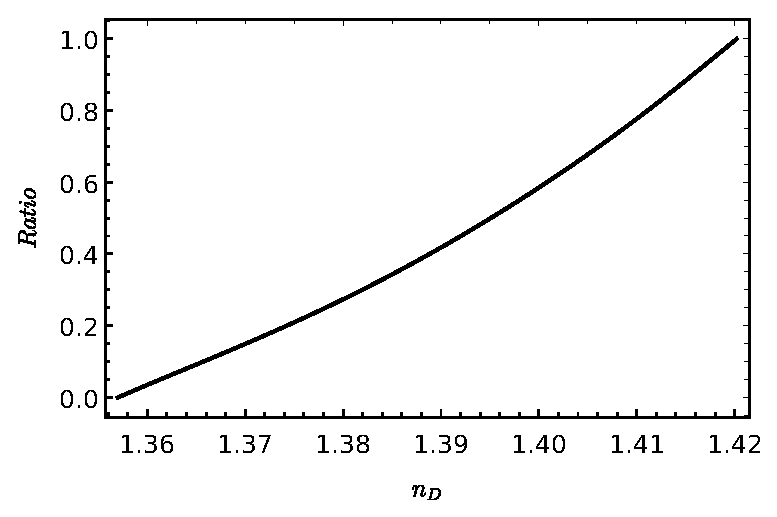
\includegraphics[width=0.45\textwidth]{figures/ethanol_cyclohexane.eps}
\caption{The curve of $n_D$ \emph{v.s.} mass ratio of cyclohexane in ethanol-cyclohexane mixture}
\label{ndratioline}
\end{figure}

\begin{figure}
\centering
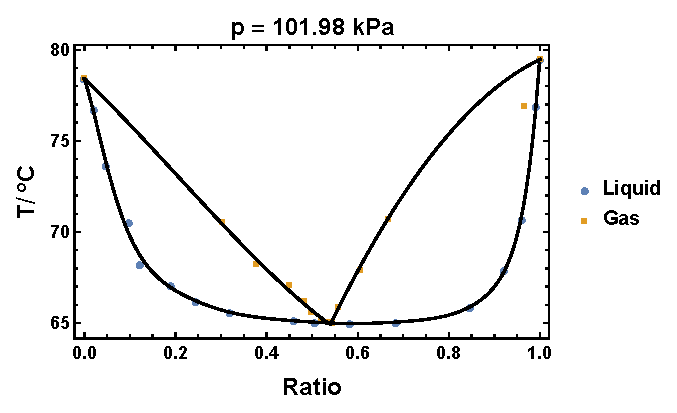
\includegraphics[width=0.45\textwidth]{figures/phasediagram.eps}
\caption{Phase diagram of ethanol-cyclohexane mixture obtained in the experiment, where `Ratio' refers to the mass ratio of cyclohexane.}
\label{phasediagram}
\end{figure}

\begin{figure}
\centering
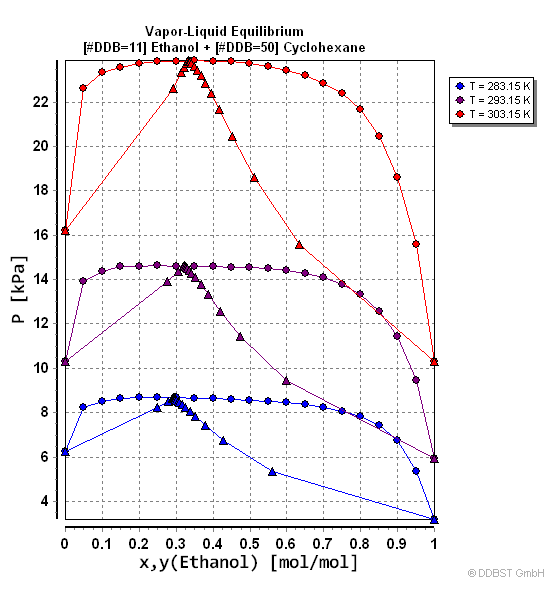
\includegraphics[width=0.45\textwidth]{figures/ECPhaseRef.png}
\caption{Phase diagram of ethanol-cyclohexane mixture from reference}
\label{phasediagramref}
\end{figure}

Fig. \ref{ndratioline} shows the relation between $n_D$ at 30 \celsius~ and the mass ratio of the cyclohexane in the ethanol-cyclohexane mixture, which is fitted by linear combination of 20 degrees of power series of $n_D$, with $R^2 = 0.99998$, verifying the result of fitting. The experiment is carried out under 101.98 kPa atmosphere pressure, the data of which is shown in Table.\ref{expdata}, and Fig.\ref{phasediagram} shows the experimental result of the ethanol-cyclohexane phase diagram, \emph{v.s.} from the reference shown in Fig.\ref{phasediagramref}\footnote{Nagai J.; Ishii N.: Parts II - IV.. J.Soc.Chem.Ind.Jap. 38 (1935) 86-10
}. The temperature is corrected according to the following formula:
\begin{equation}
\begin{cases}
\Delta t = 0.000156 h (t_1 - t_2) \\
h = t_1 - 53.82 \celsius
\end{cases}
\end{equation}
where $h$ stands for the height of the mercury exposed to room temperature, which is represented by the difference of degree of temperature. 53.82 \celsius ~refers to the graduation of the mercury thermometer at lowest point that exposed to the air.

 Similarity exists in the two phase diagrams, which indicate the validity of the experimental result, nonetheless the two diagrams are obtained under different circumstances, namely one at constant pressure, the other at constant temperature. In Fig.\ref{expdata} the lines are fitted by a linear combination of power series of the ratio perspectively, and is optimized using machine learning methods integrated in \emph{Mathematica}, which is corrected by adding terms of norms of the coefficients as a penalty function to fix overfitting problems. Maximum optimization occur when 12 degrees, 3 degrees, and 2 degrees of power series of ratio are used when fitting the liquid line, left part of the gas line, right part of the gas line respectively. Deviation of the points along the line is conspicuous, which might be attributed to the not strictly conserved pressure in the apparatus, which is brought by restricted air flow between the apparatus and the atmosphere. Uneven heating of the mixture might also account for the error, which brings dynamically unstable factors into both the measurement of temperature and the mass ratio of the two components in either gas or liquid phase. It is assumed that the liquid left over at the bottom of the condenser is equivalent to the gas phase in the mass ratio of the two components, which may not be universally valid, especially when one of the two components is significantly less contained than the other. Such a error can be magnified by the fractional distillation that occurs microscopically along the condenser. Thus it is reasonable that such an error is much more apparent at around the edges of the phase diagram, which can be indicated by Fig.\ref{expdata}.

 Considering that the boiling point of an azeotrope is either the peak or the valley of the boundaries, The fitted line can be utilized to give the boiling point of the azeotrope. The fitted line of the liquid boundary is given by
 \begin{align*}
 T = -925.661 x^{12}+172041. x^{11}-927312. 
   x^{10} \\+2.21375\times 10^6 x^9-3.04585\times 
   10^6 x^8 \\ +2.65844\times 10^6 x^7-1.52815\times 
   10^6 x^6 \\+580567. x^5-141490. x^4 \\ +20181.6 
   x^3-1177.26 x^2\\-74.3486 x+78.4263
  \end{align*}
  where $x$ stands for the mass ratio of the cyclohexane. It gives the minimum temperature of 64.9811 \celsius~ at $x=0.590127$ in the range of $[0,1]$, representing the boiling point of azetope of ethanol and cyclohexane at $p=101.98$ kPa.

 \section{Conclusion}
 Phase diagram of ethanol and cyclohexane is obtained at constant pressure of 101.98 kPa. Machine learning methods are utilized to fit the boundaries of the gas phase and liquid phase, which resembles the ones given in the references.





\end{document}
